\section{Systemarkitektur}
\label{chap:systemarkitektur}

Efter at have udarbejdet kravspecifikation, systemskitse og domain model, var der formet en idé om hvordan systemet skulle fungere. 
I det følgende beskrives systemarkitekturen for drone, webapplikation og server. 

Til systemarkitekturen er der anvendt SysML og UML diagrammer. SysML bruges til visualisering af de hardware blokke hvor UML diagrammer er anvendt til uddybning af software. Til supplering af UML diagrammer er n+1 modellen anvendt. N+1 modellen er en udviklingsmodel til software, som benytter sig af forskellige views til at illustrere og informere hvordan systemet er designet og implementeret.
 
\subsection{Blokbeskrivelser}
Det overordnede bdd på figur \ref{fig:bdd_asd} viser hvilke blokke systemet består af, samt hvilke parts blokkene indeholder.

\begin{figure}[H]
	\centering
	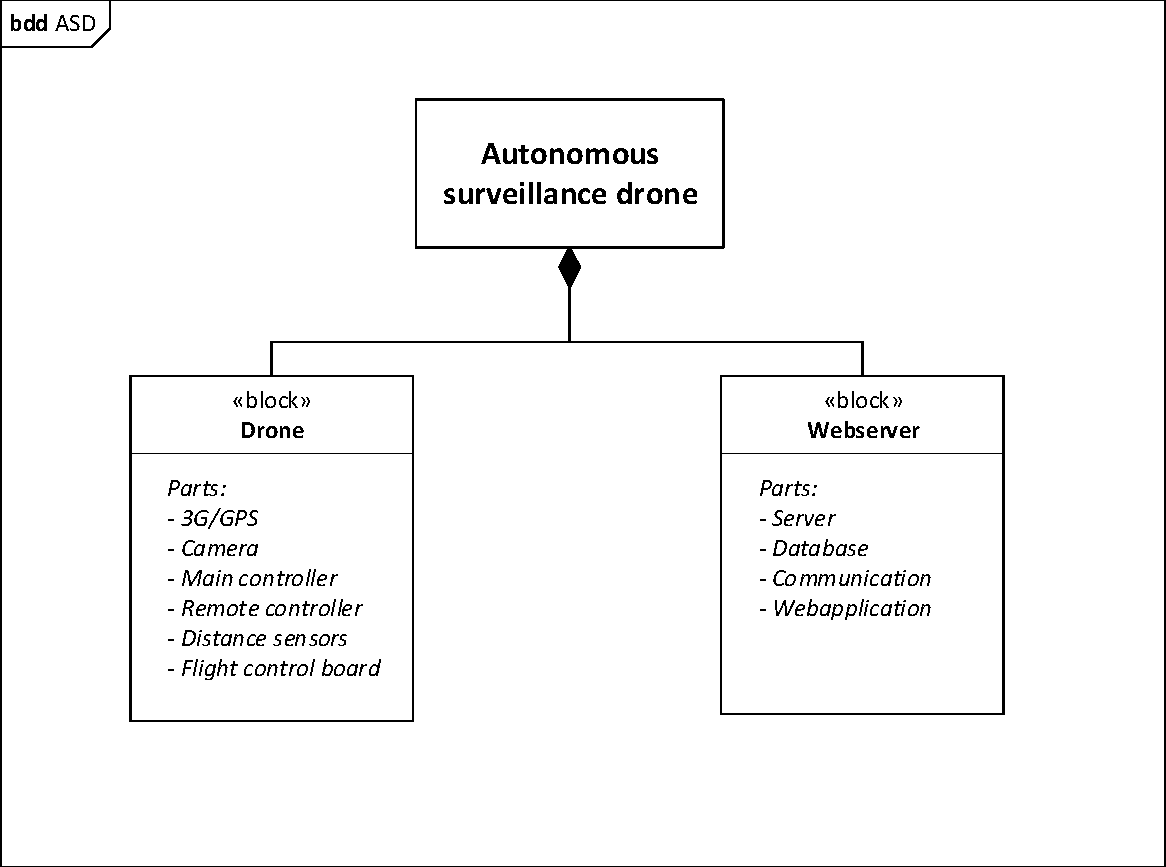
\includegraphics[width=0.80\textwidth]{Billeder/Projektbeskrivelse/bdd_overordnet.pdf}
	\caption{Overordnet bdd for systemet}
	\label{fig:bdd_asd}
\end{figure}

\textbf{Drone} \\
Drone blokken indeholder alt funktionalitet tilhørende drone. De interne forbindelse mellem de forskellige parts er beskrevet i et bdd for dronen, dette bdd kan findes i dokumentationen[X].

\textbf{Webserver} \\
Webserver blokken indeholder server, database, kommunikation og webapplikationen.

\subsection{Interne forbindelser}
\vspace{-0.3cm}	
Det overordnede ibd på figur \ref{fig:ibd_asd} beskriver hvorledes de forskellige blokke kommunikerer samt hvilken type signal der anvendes.
Denne ibd beskriver hvordan systemets største blokke kommunikerer internt og med omverdenen. 

\begin{figure}[H]
	\centering
	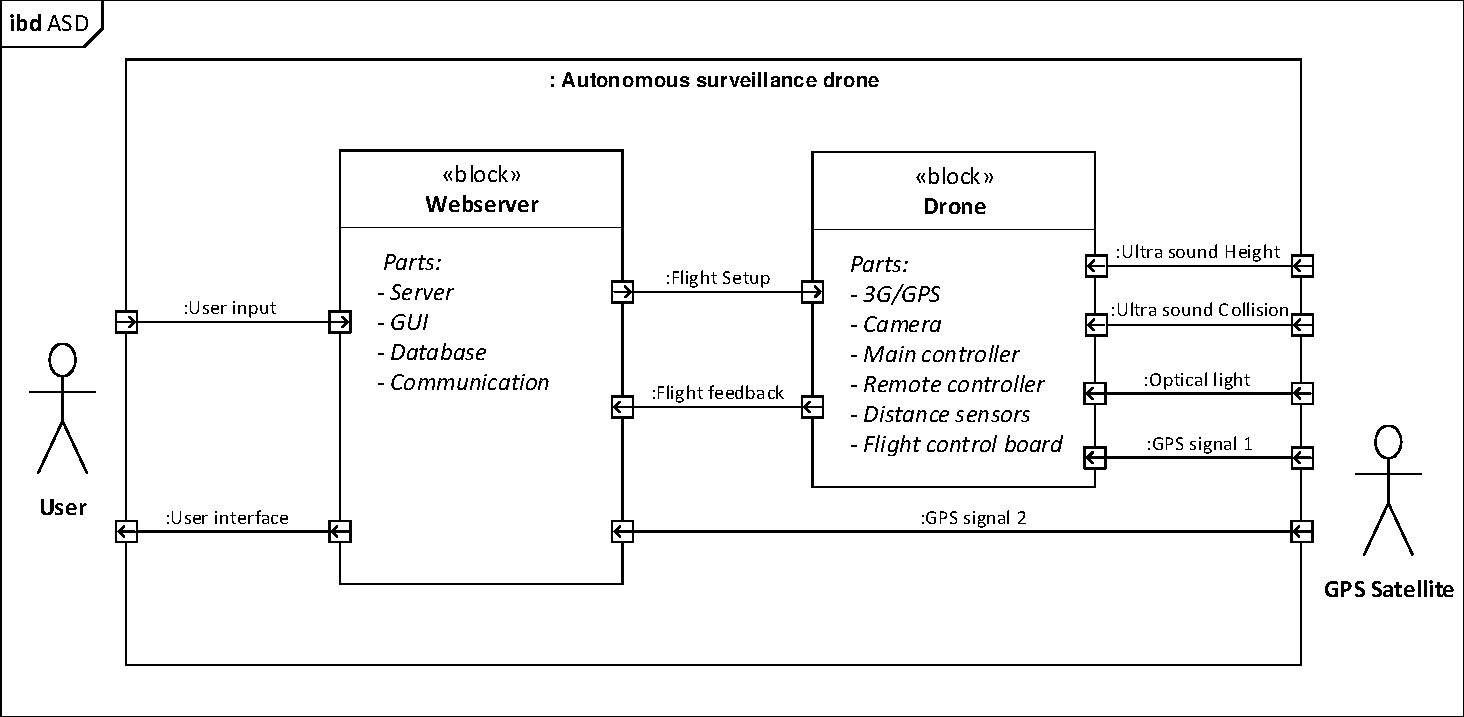
\includegraphics[width=1\textwidth]{Billeder/Projektbeskrivelse/ibd1_overordnet.pdf}
	\caption{Overordnet ibd for systemet}
	\label{fig:ibd_asd}
\end{figure}

Der er ikke nogle udvidede ibd'er for webserver, da webserveren beskrives med UML i stedet for SysML. 
For en beskrivelse af de uddybede ibd'er til drone henvises til dokumentationens systemarkitektur og design [X].

\subsection{Pakke diagram}
\vspace{-0.3cm}	
Pakkediagrammer viser hvilke ansvarsområder hver pakke har.
På figur \ref{fig:package_drone} ses de overordnede pakker der beskriver dronens opdeling og hvilke ansvars områder der er.
Pakkernes ansvarsområde danner grundlag for udformning af klasserne og klassernes indbyrdes forhold.
 
\begin{figure}[H]
	\centering
	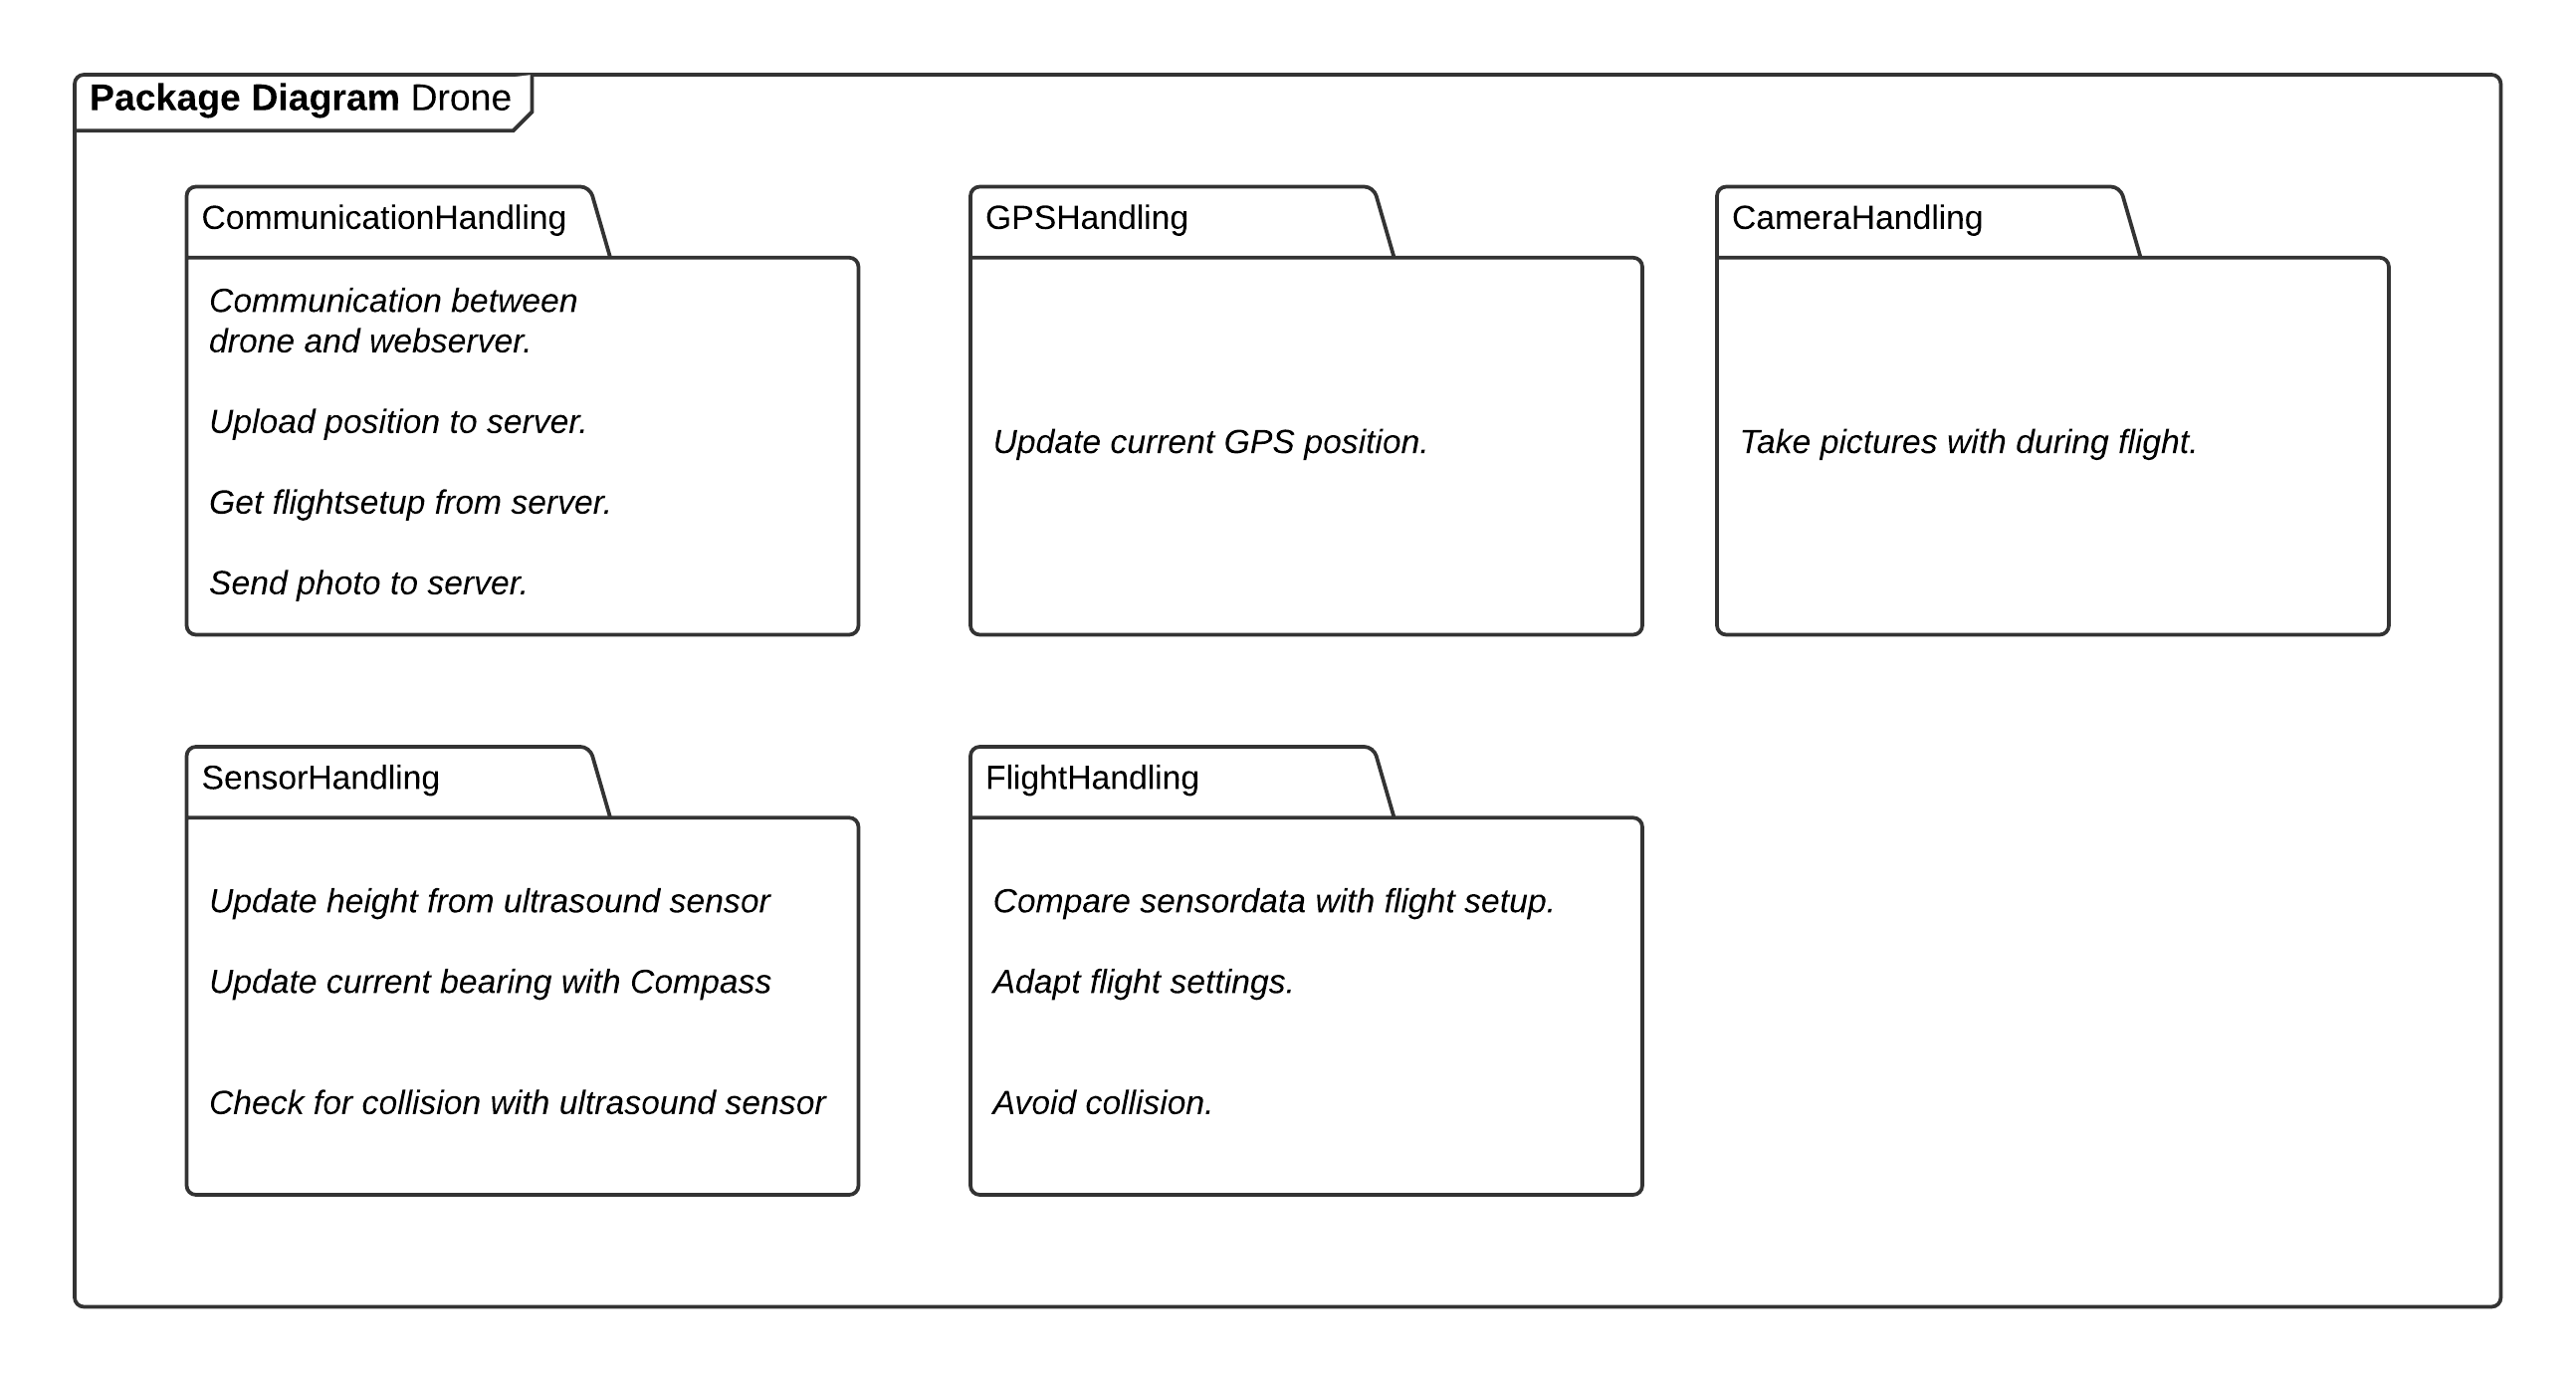
\includegraphics[width=0.85\textwidth]{Billeder/Projektbeskrivelse/Packagediagram_drone}
	\vspace{-0.3cm}	
	\caption{Overordnet pakke diagram for drone}
	\label{fig:package_drone}
\end{figure}